%%%%%%%%%%%%%%%%%%%%%%%%%%%%%%%%%%%%%%%%%%%%%%%%%%%%%%%%%%%%%%%%%%%%%%%%%%%%%%%
% Copyright 2020
% Little Compline with Akathist to the Theotokos
% as  served on the first 4 Fridays of Great Lent
%%%%%%%%%%%%%%%%%%%%%%%%%%%%%%%%%%%%%%%%%%%%%%%%%%%%%%%%%%%%%%%%%%%%%%%%%%%%%%%

\documentclass[twoside, letterpaper, 12pt]{report}
\usepackage{orthodoxservicebook}

\title{Little Compline with Akathist to the Theotokos\\
       As served on the first four Fridays of Great Lent}
\author{St. Katherine Orthodox Church}
\date{}% Remove date

\titlepic{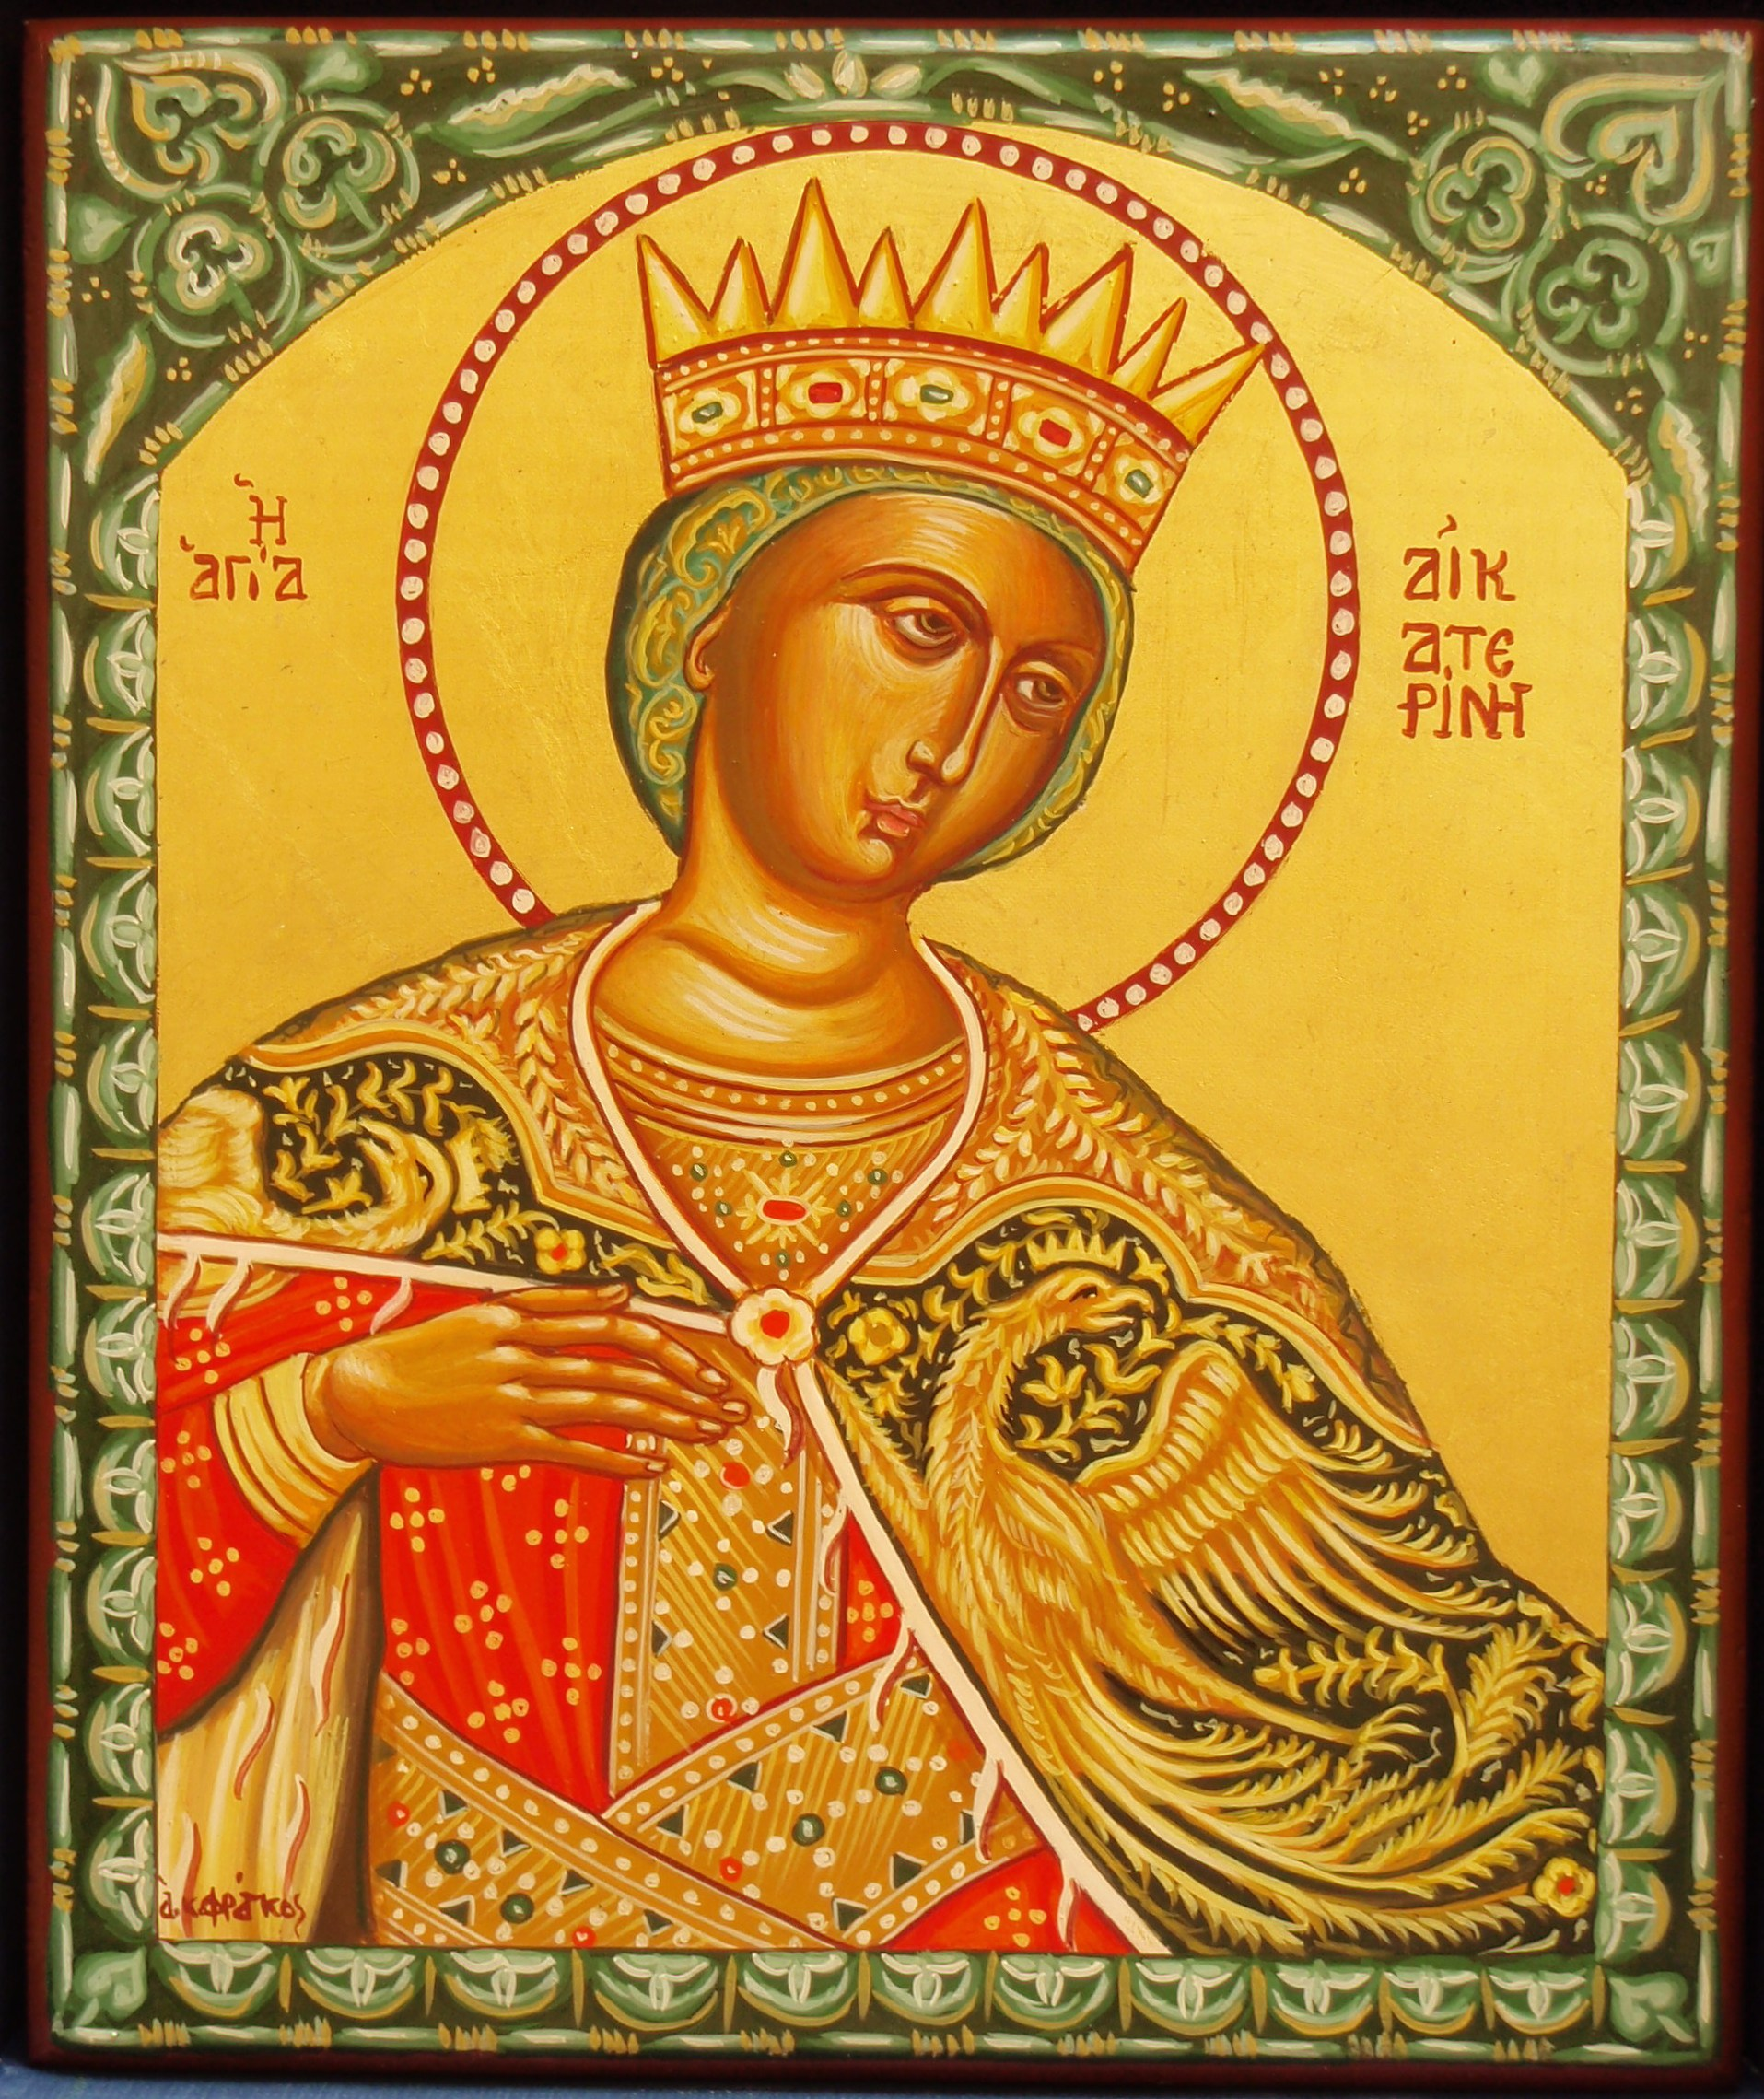
\includegraphics[width=0.5\textwidth]{Katherine1.jpg}}

\begin{document}
\maketitle
\pagestyle{empty} % Don't show page numbers

\instruction{This page intentionally left blank}

\cleardoublepage
\pagestyle{plain}
\setcounter{page}{1}

\chapter*{Little Compline, First Half}
\begin{priest}
\item Blessed is our God, always, now and ever, and unto ages of ages.
\end{priest}

\choralresponse{./Z-Responses/RussianPresanctified/Amen.ly}

\begin{priest}
\item Glory to Thee, our God. Glory to Thee.
\item O heavenly King, Comforter, the Spirit of truth,
who art everywhere present and fillest all things,
the Treasury of good things and Giver of life:
Come and abide in us and cleanse us from every stain and save our souls,
O Good One.
\end{priest}

\centeredsection{The Trisagion Prayers}
\instruction{Recited together as a congregation}

Holy God, Holy Mighty, Holy Immortal: have mercy on us. \instruction{(THRICE)}

\vbox{}
\emph{Glory to the Father, and to the Son, and to the Holy Spirit; both now and ever, and
unto ages of ages. Amen.}

\vbox{}
All-holy Trinity, have mercy on us. Lord, cleanse us from our sins. Master, pardon
our iniquities. Holy God, visit and heal our infirmities for Thy Name’s sake.

\vbox{}
Lord, have mercy. \instruction{(3x)}

\vbox{}
\emph{Glory to the Father, and to the Son, and to the Holy Spirit; both now and ever, and
unto ages of ages. Amen.}

\vbox{}
Our Father, Who art in Heaven, hallowed be Thy Name. Thy kingdom come; Thy
will be done on earth as it is in Heaven. Give us this day our daily bread; and forgive
us our trespasses, as we forgive those who trespass against us, and lead us not into
temptation, but deliver us from evil.

\begin{priest}
\item For Thine is the kingdom, and the power, and the glory:
    of the Father, and of the Son, and of the Holy Spirit; now and ever, and unto ages of ages.
\end{priest}

\choralresponse{./Z-Responses/RussianPresanctified/Amen.ly}

\begin{reader}
\item Lord, have mercy. \twelve
\item Glory to the Father, and to the Son, and to the Holy Spirit;
  both now and ever, 
  and unto ages of ages. Amen.

\item O come, let us worship and fall down before God our King.\\
  O come, let us worship and fall down before Christ, our King and our God.\\
  O come, let us worship and fall down before the Very Christ, our King and our God.
\end{reader}

\begin{maybetwocolumns}

\centeredsection{Psalm 50}
\input{Psalms/Psalm050.txt}

\centeredsection{Psalm 69}
\input{Psalms/Psalm069.txt}

\centeredsection{Psalm 142}
\input{Psalms/Psalm142.txt}

\centeredsection{The Little Doxology}
\instruction{Plain reading}
\begin{itemize}[label=\small{+},leftmargin=*]
\item Glory to God in the highest, and on earth peace, good will among men.
\item We praise Thee, we bless Thee, we worship Thee, we glorify Thee;
      we give thanks unto Thee for Thy great glory.
\item O Lord, heavenly King, God the Father Almighty;
      O Lord, the only-begotten Son, Jesus Christ; and the Holy Spirit.
\item O Lord God, Lamb of God, Son of the Father, Who takest away the sin of the world,
      have mercy on us; O Thou Who takest away the sins of the world.
\item Receive our prayer, O Thou Who sittest at the right hand of the Father,
      and have mercy on us.
\item For Thou only art holy, Thou only art the Lord, O Jesus Christ,
      to the Glory of God the Father. Amen.
\item Every day will I bless Thee, and I will praise Thy Name forever;
      yea, forever and ever.
\item Lord, Thou hast been our refuge in all generations.
      I said: Be merciful unto me; heal my soul, for I have sinned against Thee.
\item Lord, I have fled unto Thee: teach me to do Thy will, for Thou art my God.
\item For with Thee is the fountain of life: in Thy light shall we see light.
\item O continue Thy loving-kindness unto them that know Thee.
\item Vouchsafe, O Lord, to keep us this night without sin.
\item Blessed art Thou, O Lord God of our Fathers,
      and praised and glorified be Thy Name forever. Amen.
\item Let Thy mercy, O Lord: be upon us, as we do put our hope in Thee.
\item Blessed art Thou, O Lord: teach me Thy statutes.
\item Blessed art Thou, O Master; make me to understand Thy statutes.
\item Blessed art Thou, O Holy One; enlighten me with Thy statutes.
\item Thy mercy, O Lord, endureth forever.
      O despise not the works of Thy hands.
      To Thee belongeth worship, to Thee belongeth praise, to Thee belongeth glory:
      to the Father, and to the Son, and to the Holy Spirit;
      now and ever, and unto ages of ages. Amen.
\end{itemize}
\end{maybetwocolumns}

\centeredsection{The Nicene Creed}
\instruction{Recited together as a congregation}

\verbatiminput{Common/TheCreed.txt}

\squashedcenteredsection{Theotokon}
\instruction{Plain reading}

\readerline{\input{Common/ItIsTrulyMeetToBlessTheeOTheotokos.txt}}

\chapter*{The Canon of the Akathist}

\centeredsection{Ode One}
\lilypondfile{./4-Orthros/CanonOfTheAkathist-ToTheTheotokos/CanonOde1-Tone4-Kazan.ly}

\choralresponse{./Z-Responses/AkathistHymnBasil/MostHolyTheotokosSaveUs.ly}

When the great Archangel saw thee, O immaculate one,
thou living book of Christ, sealed by the Spirit, he cried unto thee:
Hail, vessel of gladness, through whom the curse of our first-mother is loosed.

\choralresponse{./Z-Responses/AkathistHymnBasil/MostHolyTheotokosSaveUs.ly}

Hail, virgin bride of God, thou uplifter of Adam and death-knell of Hades;
Hail, O all-blameless one, thou palace of the only King; Hail,
thou fiery throne of the Almighty.

\choralresponse{./Z-Responses/AkathistHymnBasil/GlorytoTheFSandHS.ly}

Hail, thou from whom alone didst blossom the Unwithering Rose;
Hail, thou who didst bear the fragrant Apple;
Hail, immaculate maiden, fragrance of the King of All and salvation of the world.

\choralresponse{./Z-Responses/AkathistHymnBasil/BothNowAndEver.ly}

Hail, thou treasure-house of purity, through which we rose up from our fall;
Hail, Lady, sweet-scented lily perfuming the faithful,
thou fragrant incense and most precious myrrh.


\centeredsection{Ode Three}

\lilypondfile{./4-Orthros/CanonOfTheAkathist-ToTheTheotokos/CanonOde3-Tone4-Kazan.ly}

\choralresponse{./Z-Responses/AkathistHymnBasil/MostHolyTheotokosSaveUs.ly}

As a clear and untilled field, thou didst make the Divine Ear of Grain to sprout;
Hail, thou living table that held the Bread of Life;
Hail, thou unfailing fountain of Living Water.

\choralresponse{./Z-Responses/AkathistHymnBasil/MostHolyTheotokosSaveUs.ly}

Hail, O mystic heifer that didst bear the Spotless Calf;
Hail, ewe-lamb who didst conceive the Lamb of God that taketh away the sins
of the whole world; Hail, thou fervent intercessor.

\choralresponse{./Z-Responses/AkathistHymnBasil/GlorytoTheFSandHS.ly}

Hail, O radiant dawn, which alone dost bear Christ the Sun, the dwelling-place of Light;
Hail, thou who didst dispel the darkness and reduce to naught the demons of gloom.

\choralresponse{./Z-Responses/AkathistHymnBasil/BothNowAndEver.ly}

Hail, thou only gate, through which the Word alone didst pass;
Hail, Lady, for by thy birth-giving the bars and gates of Hades were burst asunder;
Hail, thou most worthy of all praise, divine entry for the saved.


\centeredsection{Ode Four}

\lilypondfile{./4-Orthros/CanonOfTheAkathist-ToTheTheotokos/CanonOde4-Tone4-Kazan.ly}

\choralresponse{./Z-Responses/AkathistHymnBasil/MostHolyTheotokosSaveUs.ly}

In hymns of faith, O all-praised one, we cry out unto thee:
Hail, thou mountain fertile with the fullness of the Spirit;
Hail, thou lamp of light and vase of manna, to the senses of the reverent most sweet.

\choralresponse{./Z-Responses/AkathistHymnBasil/MostHolyTheotokosSaveUs.ly}

Hail, immaculate Lady, mercy-seat of the world;
Hail, thou ladder which raised all from earth to grace;
Hail, thou bridge which truly leads from death to life all who sing thy praises.

\choralresponse{./Z-Responses/AkathistHymnBasil/MostHolyTheotokosSaveUs.ly}

Hail, O immaculate one, higher than the heavens,
thou who didst without pain carry within thee the Foundation of the Earth.
Hail, O seashell that didst dip in thy blood the divine purple
for the King of the Powers of Heaven.

\choralresponse{./Z-Responses/AkathistHymnBasil/GlorytoTheFSandHS.ly}

Hail, Lady, who didst truly bear the Lawgiver
that freely blotted out the transgressions of all;
O unimaginable depth, O height ineffable, O maiden unwedded,
through whom we are become divine.

\choralresponse{./Z-Responses/AkathistHymnBasil/BothNowAndEver.ly}

With hymns we praise thee, O thou who didst weave for the world a crown not woven by hands;
Hail to thee, O Virgin, do we cry: fortress of all mankind,
and rampart, and strength, and refuge divine.


\centeredsection{Ode Five}

\lilypondfile{./4-Orthros/CanonOfTheAkathist-ToTheTheotokos/CanonOde5-Tone4-Kazan.ly}

\choralresponse{./Z-Responses/AkathistHymnBasil/MostHolyTheotokosSaveUs.ly}

Hail, O all-blameless one,
who didst bear the Way of Life and save the world from the deluge of sin;
Hail, bride of God, thou of great report and mighty fame;
Hail, thou dwelling-place of the Master of Creation.

\choralresponse{./Z-Responses/AkathistHymnBasil/MostHolyTheotokosSaveUs.ly}

Hail, O immaculate one, stronghold and fortress of mankind,
and place of hallowed glory, deathknell of Hades, bridal-chamber full of light;
Hail, joy of the angels;
Hail, help of those who faithfully pray unto thee.

\choralresponse{./Z-Responses/AkathistHymnBasil/MostHolyTheotokosSaveUs.ly}

Hail, O Lady, fiery chariot of the Word;
living paradise having the Lord, the Tree of Life, in thy midst;
His sweetness gives life to those who partake in faith,
even though they be subject to corruption.

\choralresponse{./Z-Responses/AkathistHymnBasil/GlorytoTheFSandHS.ly}

Strengthened by thy might, faithfully we cry unto thee:
Hail, city of the King of All, great in glory and repute,
of whom all these were clearly spoken;
O mount unhewn and depth beyond all measure.

\choralresponse{./Z-Responses/AkathistHymnBasil/BothNowAndEver.ly}

Thou spacious tabernacle of the Word,
Hail! O immaculate one, thou seashell which didst proffer the Divine Pearl;
Hail! O all-wondrous one, thou art the reconciliation to God,
O Theotokos, of all who ever bless thee.


\centeredsection{Ode Six}

\lilypondfile{./4-Orthros/CanonOfTheAkathist-ToTheTheotokos/CanonOde6-Tone4-Kazan.ly}

\choralresponse{./Z-Responses/AkathistHymnBasil/MostHolyTheotokosSaveUs.ly}

Immaculate bridal-chamber of the Word, and aid to the sanctification of us all,
Hail! O all-pure maiden, whom the Prophets did proclaim;
Hail, thou ornament of the Apostles!

\choralresponse{./Z-Responses/AkathistHymnBasil/MostHolyTheotokosSaveUs.ly}

From thee the dew distilled that quenched the flame of polytheism;
wherefore, we cry out unto thee, O Virgin:
Hail, O dewy fleece which Gideon did foresee.

\choralresponse{./Z-Responses/AkathistHymnBasil/GlorytoTheFSandHS.ly}

Behold, we cry out unto thee:
Hail! Be thou our haven and our port when we voyage
on the sea of tribulations and through the snares of the adversary

\choralresponse{./Z-Responses/AkathistHymnBasil/BothNowAndEver.ly}

O cause of joy, favor us with reason to cry out unto thee:
Hail, thou bush that burns yet unconsumed,
thou light-filled cloud which unceasingly shelters the faithful.


\centeredsection{Ode Seven}

\lilypondfile{./4-Orthros/CanonOfTheAkathist-ToTheTheotokos/CanonOde7-Tone4-Kazan.ly}

\choralresponse{./Z-Responses/AkathistHymnBasil/MostHolyTheotokosSaveUs.ly}

To thee we sing a hymn and cry: Hail! Chariot of the mystic sun,
true vine that did produce the ripe cluster of grapes,
dripping wine to gladden the souls of those who with faith do glorify thee.

\choralresponse{./Z-Responses/AkathistHymnBasil/MostHolyTheotokosSaveUs.ly}

Hail, thou Bride of God, who didst bear the Healer of Mankind;
the mystic staff from which blossomed the Unfading Flower;
Hail, O sovereign Lady, through whom we are filled with joy,
and made inheritors of life.

\choralresponse{./Z-Responses/AkathistHymnBasil/MostHolyTheotokosSaveUs.ly}

The tongue of eloquence has not power to sing thy praises,
O sovereign Lady, for thou wast exalted above the Seraphim
when thou didst bear Christ the King;
do thou now implore Him to deliver from all harm
those who faithfully reverence thee.

\choralresponse{./Z-Responses/AkathistHymnBasil/GlorytoTheFSandHS.ly}

The ends of the earth do praise and bless thee, and cry out unto thee:
Hail, pure Maiden, scroll on which the finger of God did inscribe His Word;
do thou now implore Him, O Theotokos,
to write down thy servants in the Book of Life.

\choralresponse{./Z-Responses/AkathistHymnBasil/BothNowAndEver.ly}

We thy servants bend the knee of our hearts and implore thee, O pure Maiden:
incline thine ear and save us, who are engulfed in tribulations;
and guard thy city, O Theotokos, from every assault of her enemies.

\centeredsection{Ode Eight}

\lilypondfile{./4-Orthros/CanonOfTheAkathist-ToTheTheotokos/CanonOde8-Tone4-Kazan.ly}

\choralresponse{./Z-Responses/AkathistHymnBasil/MostHolyTheotokosSaveUs.ly}

Thou didst receive the Word within thee, O pure Maiden,
and didst bear Him Who beareth all things;
thou didst nourish Him with milk, Who by His nod dost sustain all the universe;
to Him we sing: All ye works, praise the Lord, and magnify Him unto all ages.

\choralresponse{./Z-Responses/AkathistHymnBasil/MostHolyTheotokosSaveUs.ly}

Moses perceived in the burning bush the great mystery of thy birth-giving,
O chaste and holy Virgin;
the children prefigured this most clearly
when they stood in the midst of the flame and were un-burned;
wherefore, we praise thee unto all ages.

\choralresponse{./Z-Responses/AkathistHymnBasil/MostHolyTheotokosSaveUs.ly}

We, who of old were made naked by deceit,
have been clothed in a garment of incorruption by thy conception;
and we who were sitting in the darkness of transgressions
have come to see the light,
O Maiden who art the dwelling-place of Light:
wherefore, we praise thee unto all ages.

\choralresponse{./Z-Responses/AkathistHymnBasil/GlorytoTheFSandHS.ly}

Through thee the dead are made to live, for thou didst bear the Life Essential;
those who before were speechless now find useful eloquence,
lepers are cleansed, diseases are driven away,
and the multitude of aerial spirits are vanquished,
O Virgin, salvation of mortals.

\choralresponse{./Z-Responses/AkathistHymnBasil/BothNowAndEver.ly}

We hail thee, O all-blessed one,
who didst bring forth salvation for the world,
through which we have been raised from earth to heights above;
O pure Maiden, thou art shelter and stronghold,
bulwark and fortress of all who sing:
All ye works, praise the Lord, and magnify Him unto all ages.


\centeredsection{Ode Nine}

\lilypondfile{./4-Orthros/CanonOfTheAkathist-ToTheTheotokos/CanonOde9-Tone4-Kazan.ly}

\choralresponse{./Z-Responses/AkathistHymnBasil/MostHolyTheotokosSaveUs.ly}

Through thee, O Maiden, have we faithful become partakers of joy,
so that we may further cry out unto thee:
Hail! Do thou deliver us from perpetual temptation, from barbaric attack,
and from all the multitude of evils which we mortals suffer
for the number of our sins.

\choralresponse{./Z-Responses/AkathistHymnBasil/MostHolyTheotokosSaveUs.ly}

Thou hast appeared to enlighten us and be our confirmation,
wherefore we cry aloud to thee:
Hail, O unsetting star which didst introduce into the world the mighty Sun;
Hail, pure maiden, who didst open up fast-closed Eden;
Hail, fiery pillar, which doth lead man’s nature to the life above.

\choralresponse{./Z-Responses/AkathistHymnBasil/MostHolyTheotokosSaveUs.ly}

Let us stand with reverence in the house of our God, and let us cry aloud:
Hail, mistress of the world;
Hail, Mary, Lady of us all;
Hail, thou who alone art blameless among women, and beautiful;
Hail, O vessel, which didst receive into thyself the myrrh
which was never before outpoured.

\choralresponse{./Z-Responses/AkathistHymnBasil/GlorytoTheFSandHS.ly}

Hail, O Ever-virgin, thou dove who didst bring forth Him Who is merciful.
Hail, boast of all the righteous saints and crown of those who strive.
Hail, ornament divine of all the just, and of us the faithful,
our salvation as well.

\choralresponse{./Z-Responses/AkathistHymnBasil/BothNowAndEver.ly}

Spare, O God, Thine inheritance, and overlook now all our sins.
For as intercessor in Thy sight, O Christ,
there stands before Thee she that on earth conceived Thee without seed,
when in Thy Great Mercy
Thou hast willed to be shaped in a form that was not Thine own.


\chapter*{Oikoi}

\centeredsection{First Stasis - First Friday of Great Lent}

\centeredsection{Oikos}
\begin{priest}
  \item An angel chieftain was sent from heaven to say 
    “Hail!” unto the Theotokos. \thrice{}
  \item … And beholding Thee, O Lord, taking bodily form,
    he stood rapt in wonder,
    and with bodiless voice cried aloud to her in this wise:
\end{priest}

\begin{itemize}[label=\tiny{+},leftmargin=*]
\item Hail, thou, through whom joy shall shine forth; Hail, thou, through whom the curse shall be
destroyed.
\item Hail, thou restoration of fallen Adam; Hail, thou, redemption of the tears of Eve.
\item Hail, thou height untrodden by human minds; Hail, thou depth hard to scan, even for angels’
eyes.
\item Hail, thou that art a kingly throne; Hail, thou that holdest the Upholder of all.
\item Hail, thou star that showed the Sun; Hail, womb of the Divine Incarnation.
\item Hail, thou through whom Creation is renewed; Hail, thou through whom the Creator becomes
a babe.
\item Hail, O Bride without bridegroom! \instruction{The priest censes the icon.}
\end{itemize}

Choir: Hail, O Bride without bridegroom!

\centeredsection{Kontakion}

\priestline{Boldly spake the holy maiden unto Gabriel, conscious of her chastity: To my soul thy
strange message seems hard to grasp; how speakest thou of a virgin conception, crying
aloud: Alleluia! \instruction{The priest censes the icon.}}

Choir: Alleluia.

\centeredsection{Oikos}

Priest: Craving to know knowledge unknowable, the Virgin cried out unto him who ministered
unto her: From a maiden body, how may a Son be born; tell thou me! To her he spake
in fear, and thus only cried aloud:

\begin{itemize}[label=\tiny{+},leftmargin=*]
\item Hail, thou initiate of the ineffable counsel; Hail, O faith of those who pray in silence.
\item Hail, thou beginning of the miracles of Christ; Hail, thou crown of His decrees.
\item Hail, heavenly ladder, by which God came down; Hail, bridge that leadest us from earth to
Heaven.
\item Hail, thou much-talked of wonder of angels; Hail, thou much-lamented damager of demons.
\item Hail, thou who ineffably didst bear the Light; Hail, thou who told none how it was done.
\item Hail thou, who over-soarest the knowledge of the wise; Hail, thou who enlightenest the minds
of the faithful.
\item Hail, O Bride without bridegroom! \instruction{The priest censes the icon.}
\end{itemize}

Choir: Hail, O Bride without bridegroom!

\centeredsection{Kontakion}
\priestline{Divine power from on high then overshadowed the maiden, that she might conceive,
and showed forth her fruitful womb as a fertile field to all who desire to reap salvation,
as they sing: Alleluia! \instruction{The priest censes the icon.}}

Choir: Alleluia. 

\centeredsection{Oikos}
Priest: Enshrining God in her womb, the Virgin hastened unto Elizabeth; whose unborn babe
at once perceived her Salutation, and rejoiced; and with stirrings as if with voices cried
out to the Theotokos:

\begin{itemize}[label=\tiny{+},leftmargin=*]
\item Hail, branch of unfading growth; Hail, possessor of untouched fruit.
\item Hail, thou who laborest for Him Whose labor is love; Hail, thou who tendest Him Who tendeth
our life.
\item Hail, field with compassions harvest rich; Hail, table with abundance of mercies spread.
\item Hail, thou who revivest the green meadows of joy; Hail, thou who makest ready a safe haven
for souls.
\item Hail, thou accepted incense offering of intercessions; Hail, thou oblation of all the world.
\item Hail, goodwill of God towards men; Hail, access of mortals to God.
\item Hail, O Bride without bridegroom! \instruction{The priest censes the icon.}
\end{itemize}

Choir: Hail, O Bride without bridegroom!

\centeredsection{Kontakion}
\priestline{Floods of doubtful thoughts troubled the wise Joseph within, and he feared a furtive
love as he beheld thee unwed, O Blameless One; but when he learned that thy
conception was of the Holy Spirit, he said: Alleluia! \instruction{The priest censes the icon.}}

Choir: Alleluia.

\instruction{This concludes the first stasis.
Go to page \pageref{ch:LittleComplineSecondHalf} and sing the Kontakion “To Thee the Champion Leader.”}

\chapter*{Little Compline - Second Half}
\label{ch:LittleComplineSecondHalf}
\end{document}
